\lab{Linear Regression}{Linear Regression}
\label{lab:LinearRegression}

\objective{This section will introduce the basics of Linear Regression, feature selection methods, and regularization.}

\section*{Introduction to Linear Regression}
One of the first skills taught in basic algebra is to effectively plot the line $y=mx+b$ which can be done with two points. 
But what if we want to find the line that best fits a set of points?

In this case, we can use the simplest form of linear regression: \textit{Ordinary Least Squares} (\textit{OLS}). 
Given data as a set of points $D = \{ (x_1, y_1), \ldots, (x_n, y_n) \}$ we wish to find the line that best fits the data. 
The line is given by $y = mx+ b$ where $m$ and $b$ are unknown constants and $x$ and $y$ are the independent and dependent variables respectively. 
Using OLS, let \[ y_i = mx_i + b + \epsilon_i \] describe the $ith$ point in $D$ for each $i \in \{1, \ldots, n\}$.
Note that $\epsilon_i$ is the vertical distance from the $ith$ point to the line given by $y = mx + b$ and is often called the \textit{residual} or the \textit{error}.

The $n$ equations for each point in $D$ can be written in vector notation. 
Let the $x$ and $y$ coordinates of $D$ be represented by column vectors $\boldsymbol x$ and $\boldsymbol y$ respectively.
In statistical science, the intercept ($b$) and slope ($m$) are denoted as $\beta_0$ and $\beta_1$ respectively and 
\[ \begin{bmatrix} b \\ m \end{bmatrix} = \begin{bmatrix} \beta_0 \\ \beta_1 \end{bmatrix} = \boldsymbol\beta .\]
Additionally, the residuals are represented by a column vector  $\boldsymbol\epsilon$ and $\boldsymbol 1$ is a column vector of ones. 
So we have \[ \boldsymbol y = m \boldsymbol x + \boldsymbol 1 b + \boldsymbol\epsilon = [\boldsymbol 1, \boldsymbol x] \cdot \begin{bmatrix} b \\ m \end{bmatrix} + \boldsymbol\epsilon. \]
Denoting $X = [ \boldsymbol 1, \boldsymbol x ]$, we have our final equation given as \[ \boldsymbol y = X \boldsymbol\beta + \boldsymbol\epsilon . \]
This notation may seem excessive, but suppose we wanted to fit a model of the form $y=ax^3 + bx^2 + cx+d$
A little work can show that $X=[ \boldsymbol 1,\boldsymbol x, \boldsymbol x^2, \boldsymbol x^3]$ and $\boldsymbol\beta = [\beta_0, \beta_1, \beta_2, \beta_3]^T$, which is very easy to work with.
Thus, this notation is actually the ideal way to generalize linear regression, especially when working with higher degree polynomials.

The solution to OLS is straight forward with some important assumptions. Sparing you the algebraic details and assuming that 
$\boldsymbol y \sim \mathcal{N}(X\boldsymbol\beta, \sigma^2 \boldsymbol I)$ and $\boldsymbol\epsilon \sim \mathcal{N}(\boldsymbol 0, \sigma^2 \boldsymbol I)$ and $\boldsymbol I$ is the identity matrix, 
the least squares estimator for $\boldsymbol\beta$ is given as 
\begin{equation}
\widehat{\boldsymbol\beta} = (X^TX)^{-1} X^T \boldsymbol y .
\end{equation}

\begin{problem}
Write a function that takes as input \li{X} and \li{y}. In your function, add a column of ones to \li{X} to account for $\beta_0$. Call this function \li{ols}. This function should return the least squares estimator for $\boldsymbol\beta$ as a numpy array.

Hint: Try rearranging equation $1.1$ and use \li{np.linalg.solve()} to avoid inverting $(X^T X)$.
\end{problem}

\begin{problem}
Use the following code to generate random data.
\begin{lstlisting}
n = 100 # Number of points to generate
X = np.arange(100) # The input X for the function ols
eps = np.random.uniform(-10,10, size=(100,)) # Noise to generate random y coordinates
y = .3*X + 3 + eps # The input y for the function ols
\end{lstlisting} 
Find the least squares estimator for $\boldsymbol\beta$ using this random data. 
Produce a plot showing the random data and the line of best fit determined by the least squares estimator for $\boldsymbol\beta$. 
Your plot should include a title, axis labels, and a legend. 
\end{problem}

\section*{Rank-Deficient Models}
Notice that in order to find the least squares estimator $\widehat{\boldsymbol\beta}$, we need $X^TX$ to be invertible. 
However, when $X$ does not have full rank, the product $X^TX$ is singular and not invertible. 
We can no longer use the previous solution for the least squares estimator, but we can use the SVD and still compute a solution. 

Recall that if $X \in M_{n\times d}$ has rank $r$, then the compact form of the SVD of $X$ is \[ X = U\Sigma V^H \]
where $U \in M_{n\times r}$ and $V \in M_{r\times d}$ have orthonormal columns and $\Sigma \in M_{r\times r}$ is diagonal. 
In addition, if $X$ is real, then the factors $U$, $\Sigma$, and $V^H$ are also real. In this lab we assume $X$ is real. 
As described in Volume 1, there is a unique solution for the least squares estimator given by 
\begin{equation}
\widehat{\boldsymbol\beta} = V \Sigma^{-1}U^T\boldsymbol y. 
\end{equation}

\begin{problem}
Write a function that finds the least squares estimator for rank-deficient models using the SVD. 
The function should still take \li{X} and \li{y} as inputs. In your function, add a column of ones to \li{X} to account for $\beta_0$. Call the function \li{svd_ols} and return the least squares estimator for $\boldsymbol\beta$ as a numpy array.

Hint: Use \li{np.linalg.svd} to factor \li{X} and use the argument \li{full_matrices=False}. Consider solving for $\Sigma^{-1}$ using the command, \li{np.diag(1/s)}, where \li{s} is the second thing being returned in \li{np.linalg.svd}.  
\end{problem}

\begin{problem}
Use the following code to generate random data:
\begin{lstlisting}
x = np.linspace(-4, 2, 500)
y = x**3 + 3*x**2 - x - 3.5 
eps = np.random.normal(0, 3, len(y)) # Create noise 
y += eps # Add noise to randomize data
\end{lstlisting} 
Now use your function \li{svd_ols} to find the least squares estimator for a cubic polynomial. 
This can be done by passing in $X=[\boldsymbol x, \boldsymbol x^2, \boldsymbol x^3]$ into \li{svd_ols}.
Create a plot that shows a scatter plot of the data and a curve using the least squares estimator. 
Your plot should include a title, axis labels, a legend, and should look similar to Figure \ref{fig:prob4}.
\end{problem}

\begin{figure}[H]
    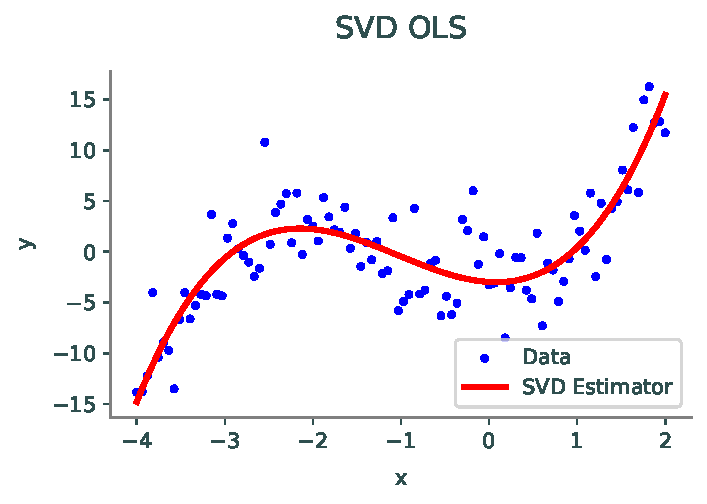
\includegraphics[width=.7\textwidth]{figures/cubic_polynomial.pdf}
    \caption{This is the SVD estimator for a cubic polynomial.}
    \label{fig:prob4}
\end{figure}

%%%
%\section*{Multiple Linear Regression}
%
%So far we have been able to graph our data and plot a line of best fit produced by the least squares estimator. 
%However, any given realistic problem can have more than one independent variable. 
%Multiple linear regression simply occurs when there are multiple independent variables used to predict the outcome of the dependent variable. 
%It is often difficult or impossible to visualize results of multiple linear regression with a line of best fit, but we still need to determine if a model is good or not.
%%%

\section*{Model Accuracy}

\subsection*{Residual Sum of Squares}
The \textit{Residual Sum of Squares} (\textit{RSS}) is a common choice of measure for the quality of a model. 
The formula for $RSS$ is given by \[ RSS = \vert\vert \boldsymbol y - X\widehat{\boldsymbol\beta} \vert\vert _2^2. \]
Notice that the $RSS$ measures the variance in the error of the model. So relative to other models, a smaller $RSS$ value indicates a more accurate model. 

\subsection*{Coefficient of Determination}
Another method of model accuracy is the \textit{Coefficient of Determination}, denoted $R^2$. In the case of linear regression, 
\[ R^2 =1 - \frac{RSS}{\sum_{i=1}^n(y_i - \bar{y})^2} \] 
and $\bar{y}= \frac{1}{n}\sum_{i=1}^n y_i$ is the sample mean of $\boldsymbol y$.
The intuition of $R^2$ is that the ratio of the average residual and biased sample variance of $\boldsymbol y$ is approximately the total variance explained by the model. 
A larger $R^2$ corresponds to a model that fits better. However, $R^2$ comes with flaws such as being able to take negative values, rewarding overfitting, and punishng under-fit models.
Because of this, we typically want to use other methods for model accuracy. 

\section*{Python Example}
There are various python packages that can be used to calculate $R^2$, but we will use \li{statsmodels} in this lab. 
Below is an example of how to build a model and extract $R^2$ using \li{statsmodels}.

\begin{lstlisting}
import statsmodels.api as sm
data = pd.read_csv("/filepath") # Read in data as pandas dataframe
y = data["dependent_variable"] # Extract dependent variable
temp_X = data[["var_1", ..., "var_n"]] # Extract independent variables
X = sm.add_constant(temp_X) # Add column of 1's
model = sm.OLS(y, X).fit() # Fit the linear regression model
print(model.rsquared) # Print the R squared value
\end{lstlisting}

\begin{problem}
The file \li{realestate.csv} contains transaction data from 2012-2013. 
It has columns for transaction data, house age, distance to nearest MRT station, number of convenience stores, latitude, longitude, and house price of unit area. \footnote{See \url{https://www.kaggle.com/datasets/quantbruce/real-estate-price-prediction?resource=download}.}
Each row in the array is a separate measurement.
As independent variables, use \li{house age}, \li{distance to the nearest MRT station}, \li{number of convenience stores}, \li{latitude}, and \li{longitude}.

Find the combination of independent variables that builds the model with the best $R^2$ value when predicting \li{house price of unit area}, the dependent variable. Use \li{statsmodels} to build each model and calculate $R^2$.
Using the same combination of variables, time the methods \li{ols}, \li{svd_ols}, and \li{statsmodels}. 
Return a list with the first element being a tuple of times for each method and the second element being the best $R^2$ value from the first part of the problem.

Note that $R^2$ cannot get worse by adding more columns and also rewards overfitting, so solving for the $R^2$ value isn't the greatest in practice. The purpose of this problem is to explore the issues of using $R^2$. 

Hint: The \li{combinations} method from the \li{itertools} package will be very helpful for finding all feature combinations. 
\end{problem}

\section*{Feature Selection}

Every regression model consists of features or variables used to predict a dependent variable or result. 
An important question to ask when building regression models is, which features are the most important in predicting the dependent variable?
In addition to being used for model accuracy, $R^2$ can also be used in feature selection, as it was in Problem 5. 
It still has the same pitfalls of rewarding overfitting and punishing under-fit models, but it can be a useful tool used in conjunction with the following tools for feature selection.
While there are other methods for implementing feature selection, most incorporate the p-value and are not included in this lab. 

\subsection*{Akaike's Information Criterion (AIC)}
A simple motivation for AIC is based on balancing goodness of fit and prescribing a penalty for model complexity. 
A more rigorous motivation for AIC is given in Volume 3 using the \textit{Kullback-Leibler} (KL) divergence. 
Given two models, $f$ and $g$, the KL divergence is given by \[ KL(f,g) = \int f(z)\log \bigg(\frac{f(z)}{g(z)} \bigg)dz \] and it measures the amount of information lost when $g$ is used to model $f$. 
Thus, a lower AIC value indicates a better model.
Additionally, AIC penalizes the size of the parameter space with a coefficient of 2 which allows for slightly more complex models.


\subsection*{Bayesian Information Criterion (BIC)}  
Instead of estimating the KL-divergence between the model in question and the true model, BIC has the property of being minimized precisely when the posterior probability of a model, given the data, is maximized.
The equations for AIC and BIC only differ with one term: the coefficient weighting the size of the parameter space. The coefficient for BIC is $log(n)$ which is generally much larger than 2. 
As a result, BIC penalizes complex models more than AIC. The difference in AIC and BIC values will grow from having more data points. 

When using AIC or BIC for feature selection, you need to consider how you want to penalize features in your model. 
If you want to exclude irrelevant features, then use BIC. If you want to keep all features that are relevant, then use AIC. 
In other words, BIC is more likely to choose too small a model, and AIC is more likely to choose too large a model.

\subsection*{Python Example}
There are multiple ways to calculate AIC and BIC with various python packages.
We will use the package \li{statsmodels} for the following problem. 
When constructing $X$ for \li{statsmodels}, do not add the column of 1's manually because \li{statsmodels} has a method that will do this for us.
\begin{lstlisting}
import statsmodels.api as sm
data = pd.read_csv("/filepath") # Read in data as pandas dataframe
y = data["dependent_variable"] # Extract dependent variable 
temp_X = data[["var_1", ..., "var_n"]] # Extract independent variables 
X = sm.add_constant(temp_X) # Add column of 1's
model = sm.OLS(y, X).fit() # Fit the linear regression model
print(model.aic) # or print(model.bic)
\end{lstlisting} 

\begin{problem}
Use the file \li{realestate.csv} and the Python Example above as a template for constructing \li{y} and \li{X} and calculating model AIC and BIC. 
For the dependent variable, use \li{house price of unit area}. 
For the independent variables, use \li{house age}, \li{distance to the nearest MRT station}, \li{number of convenience stores}, \li{latitude}, and \li{longitude}.
Loop through all of the combinations of these variables and create \li{OLS} models for each of these combinations.
Solve for the \li{AIC} and \li{BIC} for each of these models.

Find the model that has the lowest AIC and the model that has the lowest BIC. Are they the same model? Print the features of the model with the lowest AIC as a list.

Hint: The \li{combinations} method from the \li{itertools} package will be very helpful for finding all feature combinations. 
\end{problem}

\section*{Regularization}
Up to this point, we have been solving the problem \[ \min_{\boldsymbol\beta} \vert\vert X\boldsymbol\beta - \boldsymbol y \vert\vert_2^2. \]
However, we have also assumed independence among the features used to predict the dependent variable. 
The pitfall of multicollinearity arises when the features of $X$ have dependence and $X$ becomes nearly singular.
As a result, the least squares estimator is susceptible to random noise or error. 
Multicollinearity typically occurs when data is collected with poor experimental design. 
It is important to have good experimental design, but regularization can be used to mitigate poor design. 
Another issue OLS faces is feature selection. 
While there are feature selection methods available, regularization can be used to minimize non-zero coefficients. 

\subsection*{Ridge Regularization Regression}
The problem posed by \textit{Ridge Regularization} is \[ \min_{\boldsymbol\beta} \vert\vert X\boldsymbol\beta - \boldsymbol y \vert\vert_2^2 + \alpha \vert\vert \boldsymbol\beta \vert\vert_2^2 \]
where $\alpha \geq 0$. This essentially penalizes the size of the coefficients.
The larger $\alpha$ is, the more the model resists multicollinearity. 

\subsection*{Lasso Regularization Regression}
The problem posed by \textit{Lasso Regularization} is \[ \min_{\boldsymbol\beta} \frac{1}{n} \vert\vert X\boldsymbol\beta - \boldsymbol y \vert\vert_2^2 + \alpha \vert\vert \boldsymbol\beta \vert\vert_1. \]
Note that $\alpha$ provides the same functionality here as it does in Ridge Regularization. However, the use of the 1-norm often results in sparse solutions. 
As a result, Lasso Regularization can be used for feature selection since it only includes the most important features.

\subsection*{Python Example}
Since $\alpha$ is not a fixed value in Ridge and Lasso Regularization, it is best practice to perform a GridSearch to find the best parameter value. 
The example below goes over the syntax for implementing Ridge Regularization. Note that the syntax for Lasso Regularization is similar.

\begin{lstlisting}
>>> from sklearn import linear_model
>>> y = # dependent variable data
>>> X = # independent variable data with no column of ones
>>> reg = linear_model.RidgeCV(alphas=np.logspace(-6, 6, 13)) # Range for grid search 
>>> reg.fit(X, y) # Fit the model
>>> reg.alpha_ # Best parameter value 
\end{lstlisting} 


\begin{problem}
Use Ridge and Lasso Regression to model \li{house price of unit area} from the file \li{realestate.csv}. 
First, do a grid search for the model parameter for both the Ridge and the Lasso models, separately.
Note that the objects \li{RidgeCV} and \li{LassoCV} have built in cross-validation.
Be sure to pass in \li{alphas=np.logspace(-6, 6, 13)} as grid parameters for each of the models. 
Then use the grid search result to fit each model.
Once you have fit the model, you can use the \li{score} method to get $R^2$. 
Print $R^2$ for each model as a tuple. 
\end{problem}






